\documentclass[11pt,letterpaper]{article}
\usepackage[lmargin=1in,rmargin=1in,bmargin=1in,tmargin=1in]{geometry}
\usepackage{style/quiz}
\usepackage{style/commands}

% -------------------
% Content
% -------------------
\begin{document}
\thispagestyle{title}

% Quiz 1
\quizsol \textit{True/False}: Prunella is trying to find the cardinality of the set $\{ 1, 2, 1, 4, 1, 8 \}$. She counts how many numbers are in the set and finds that there are six numbers. Therefore, the cardinality of the set is 6. \pspace

\sol The statement is \textit{false}. The cardinality (or `size') of a set is the number of elements in a set. However, the order of elements of a set does not matter nor do repeats within a set. Therefore, the set $\{ 1, 2, 1, 4, 1, 8 \}$ is the same as the set $\{ 1, 2, 4, 8 \}$. The cardinality of this set is clearly 4. We may then more clearly define the cardinality of a set to be the number of \textit{distinct} elements of a set. Prunella is mistaken believing that the repeated 1s count towards the cardinality. \pvspace{1.3cm}



% Quiz 2
\quizsol \textit{True/False}: If $A$ is a set with $5$ elements and $B$ is a set with $3$ elements, then $A - B$ is a set with $2$ elements. \pspace

\sol The statement is \textit{false}. It may be possible for some sets. For instance, if $A= \{ a, b, c, d, e \}$ and $B= \{ a, c, e \}$, then $A - B= \{ b, d \}$. Then $|A|= 5$, $|B|= 3$, and $|A - B|= 2$. However, this is not true for \textit{all} sets. For instance, if $A= \{ a, b, c, d, e \}$ and $B= \{ -5, 6, \text{`nice'} \}$, then $A - B= \{ a, b, c, d, e \}$. But then in this case, $|A|= 5$, $|B|= 3$, and $|A - B|= 5$. The cardinality of $A - B$ depends on how many elements of $A$ have been `removed' because they were elements of $B$. This could be 1, 2, or 3 elements depending on the cardinality of $A \cap B$. \pvspace{1.3cm}



% Quiz 3
\quizsol \textit{True/False}: The number of ways of choosing three distinct candle sticks from a collection of five to arrange on a mantle is $_5P_3= 5 \cdot 4 \cdot 3= 60$ possible choices of arrangements. \pspace

\sol The statement is \textit{true}. We can count this directly. There are 5 possible candlesticks to choose for the far left position. This leaves 4 possible choices for the rightmost candlestick and then finally 3 possible choices for the middle candlestick. But then in total there are $5 \cdot 4 \cdot 3= 60$ total possible arrangements. Alternatively, we know the number of ways of arranging $k$ objects from a collection of $n$ distinct objects, with repetition not allowed, where the order of the arrangement matters, is given by $_n P_k$. Here, we have $n= 5$ and $k= 3$. But then we know the number of possible arrangements is $_5 P_3= \frac{5!}{(5 - 3)!}= \dfrac{5!}{2!}= \frac{5 \cdot 4 \cdot 3 \cdot 2 \cdot 1}{2 \cdot 1}= 5 \cdot 4 \cdot 3= 60$. \pvspace{1.3cm}



% Quiz 4
\quizsol \textit{True/False}: The number of possible ways of guessing the correct answers to a 10~question True/False exam is $_{10}C_{10}$. \pspace

\sol The statement is \textit{false}. We know that the order of the answer choices matters. We know also that $_{10}C_{10}$ represents a combination. For combinations, order is unimportant. Therefore, it is highly unlikely (but not strictly speaking impossible) that $_{10}C_{10}$ gives the correct count. We know each question has 2 possible answers. One must answer the first question, and the second, and the third, etc. There are 10 questions. Therefore, there are $2 \cdot 2 \cdot \cdots \cdot 2= 2^{10}= 1024$ total possible number of ways of answering (guessing) the answers for this collection of 10 true/false questions. \pvspace{1.3cm}



% Quiz 5
\quizsol \textit{True/False}: Harriet lives In Alkonost, AZ. There it is sunny 90\% of the time. Harriet is planning her weekend. She can expect that there is a $0.90 \cdot 0.90= 0.81$ probability, i.e. $81\%$ chance, that it is sunny both days. \pspace

\sol The statement is \textit{false}. If $A$ and $B$ are events, then we know that $P(A \text{ and } B)= P(A) \cdot P(B)$, if $A$ and $B$ are independent. Recall two events are independent if and only if the occurrence or non-occurrence of an event changes the probability that the other event occurs/does not occur. If $A$ and $B$ are not independent, it may not be true that $P(A \text{ and } B)= P(A) \cdot P(B)$. Let $A$ be the event that it is sunny on Saturday and $B$ be the event that it is sunny on Sunday. Clearly, $A$ and $B$ are not independent events. For instance, if it is sunny/rainy one day, it is more/less likely to be sunny/rainy the next. Therefore, it may not be the case that there is a $0.90 \cdot 0.90= 0.81$ probability, i.e. $81\%$ chance, that it is sunny both days. Generally, $P(A \text{ and } B)= P(A) P(B \;|\; A)= P(B) P(A \;|\; B)$, whether or not $A$ and $B$ are independent. \pvspace{1.3cm}



% Quiz 6
\quizsol \textit{True/False}: At a community college, 45\% of students have some experience with Excel, 55\% of students have some experience with Word, and 70\% of students have experience with at least one of them. Therefore, 15\% of students have experience only with Excel. \pspace

\sol The statement is \textit{true}. If $A$ and $B$ are events, we know that $P(A \text{ or } B)= P(A) + P(B) - P(A \cap B)$. But then we know that $P(\text{Excel or Word})= P(\text{Excel}) + P(\text{Word}) - P(\text{Excel \& Word})$. But then we have $0.70= 0.45 + 0.55 - P(\text{Excel \& Word})$. Then $0.70= 1.00 - P(\text{Excel \& Word})$ so that $P(\text{Excel \& Word})= 0.30$. Finally, because every person that knows Excel either knows word or does not (and these are mutually exclusive), we know that $0.45= P(\text{Excel})= P(\text{Only Excel}) + P(\text{Excel and Word})= P(\text{Only Excel}) + 0.30$. But this shows that $P(\text{Only Excel})= 0.15$. Therefore, 15\% of students have experience only with Excel. \pvspace{1.3cm}



% Quiz 7
\quizsol \textit{True/False}:  One can use a histogram to give the number of people enjoying certain film genres. \pspace

\sol The statement is \textit{false}. A histogram is used to display counts (for ranges of values) for \textit{quantitative} data while a bar graph is used to display counts for qualitative data. Therefore, a bar graph would (or at least could) be used to display the number of people enjoying certain film genres. \pvspace{1.3cm}



% Quiz 8
\quizsol \textit{True/False}: Both mean and median are measures of center for data. \pspace

\sol The statement is \textit{true}. The mean is a measure of a center for data. The mean of a set of numbers $\{ x_1, x_2, \ldots, x_n \}$ is given by\dots
	\[
	\overline{x}= \dfrac{\sum x_i}{n}= \dfrac{x_1 + x_2 + \cdots + x_n}{n}
	\]
The median is also a measure of center for data. The median of a set of data splits the data `in half' and is the $m$th data value in the data set (when placed in ascending order), where $m$ is the smallest integer larger than $\frac{n}{2}$, if $n$ is odd. If $n$ is even, then the median is the average of the $\frac{n}{2}$th and $(\frac{n}{2} + 1)$th value in the data (when placed in ascending order). Note that the mean is \textit{not} a robust measure of center while the median is a robust measure of center; that is, the mean is `sensitive' to outliers while the median is not. \pvspace{1.1cm}



% Quiz 9
\quizsol \textit{True/False}: If the standard deviation of a finite set of data is 0, then it must be that every number in the data set is the same. \pspace

\sol The statement is \textit{true}. Recall that the standard deviation is a measure of `spread' for a dataset. Intuitively, for the standard deviation to be zero, the data must not be `spread out' at all. It would then make sense that all the numbers of the dataset must be identical. Concretely, recall that the standard deviation for a finite dataset is given by\dots
	\[
	\sigma= \sqrt{\dfrac{\sum_i (x_i - \overline{x})^2}{n - 1}}
	\]
where the dataset is $\{ x_i \}$, $n$ is the number of values in the dataset, and $\overline{x}$ is the mean of the dataset. Setting this to $0$, we have\dots
	\[
	\begin{aligned}
	\sigma&= 0 \\[0.3cm]
	\sqrt{\dfrac{\sum_i (x_i - \overline{x})^2}{n - 1}}&= 0 \\[0.3cm]
	\dfrac{\sum_i (x_i - \overline{x})^2}{n - 1}&= 0  \\[0.3cm]
	\sum_i (x_i - \overline{x})^2&= 0 
	\end{aligned}
	\]
But because $(x_i - \overline{x})^2 \geq 0$, this is a sum of nonnegative numbers. The only way for the sum to be 0 is if all the terms of the sum are equal to 0. But then $x_i - \overline{x}= 0$ for all $i$, which implies that $x_i= \overline{x}$ for all $i$. But then every number in the dataset is equal to the mean, and hence to each other. \pvspace{1.1cm}



% Quiz 10
\quizsol \textit{True/False}: Suppose you plot a normal distribution with mean $\mu$ and standard deviation $\sigma$, i.e. $N(\mu, \sigma)$. If you were to plot a normal distribution with smaller mean but larger standard deviation, this distribution would be located ‘to the left’ and would be ‘wider’ than the original distribution. \pspace

\sol The statement is \textit{true}. The mean of a normal distribution is its `center.' The larger the mean, $\mu$, the further to the right on a number line the `center' of the normal distribution appears. The standard deviation, $\sigma$, measures the `spread' of the distribution. The larger the standard deviation, the `wider' (and flatter) the distribution is. So compared to a distribution with larger mean and smaller standard deviation, i.e. another distribution with smaller mean and larger standard deviation, would have a `center' appearing to the left of the distribution and would be more `spread out' and `flatter.' We can see an example of this below (with the `original' distribution shown in black and the distribution with smaller mean and larger standard deviation shown in red).
 
	\[
	\fbox{
	\begin{tikzpicture}[scale=2,every node/.style={scale=0.5}]
	\begin{axis}[
%	grid=both,
	axis lines=middle,
	ticklabel style={fill=blue!5!white},
	axis y line= none,
	xmin= -10.5, xmax=10.5,
	ymin= -0.5, ymax=0.5,
	xtick={-10,-8,...,10},
	ytick={-10,-8,...,10},
	minor x tick num = 1,
	minor y tick num = 1,
%	xlabel=\(x\),ylabel=\(y\),
	]
	\addplot[line width=0.03cm,domain=-10:10,samples=100] {gauss(4,1)};
	\addplot[red,line width=0.03cm,domain=-10:10,samples=100] {gauss(-2.5,3)};
	\end{axis}
	\end{tikzpicture}
	}
	\] \pvspace{1.3cm}



% Quiz 11
\quizsol \textit{True/False}: If three lines intersect, they are concurrent lines. \pspace

\sol The statement is \textit{false}. Lines are concurrent if they \textit{all} share the same intersection point. However, three lines can all (mutually) intersect without sharing a common intersection point. For instance, the three lines on the left below all (pairwise) intersect but are \textit{not} concurrent while the three lines on the right below all (pairwise) intersect and \textit{are} concurrent. 
	\[
	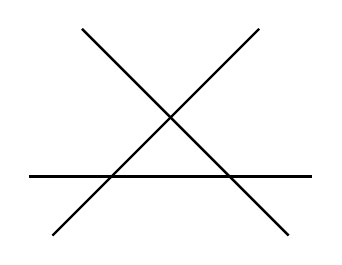
\begin{tikzpicture}[scale=1.5]
	\draw[line width= 0.03cm] (-0.75,1.25) -- (1,-0.5);
	\draw[line width= 0.03cm] (0.75,1.25) -- (-1,-0.5);
	\draw[line width= 0.03cm] (-1.2,0) -- (1.2,0);
	\end{tikzpicture}
	\hspace{4cm}
	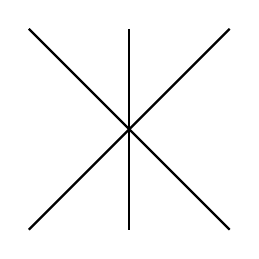
\begin{tikzpicture}[scale=1.5]
	\draw[line width= 0.03cm] (-0.85,-0.85) -- (0.85,0.85);
	\draw[line width= 0.03cm] (-0.85,0.85) -- (0.85,-0.85);
	\draw[line width= 0.03cm] (0,0.85) -- (0,-0.85);
	\end{tikzpicture}
	\] \pvspace{1.3cm}



% Quiz 12
\quizsol \textit{True/False}: There exists a right triangle with external angle 30$^\circ$. \pspace

\sol The statement is \textit{false}. If there were such a right triangle, we could create a picture like the given below.
	\[
	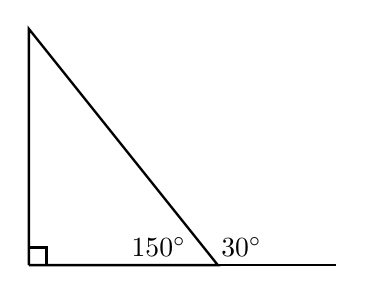
\begin{tikzpicture}[scale=1.5]
	\draw[line width= 0.03cm] (0,0) -- (0,2) -- (1.6,0) -- (0,0);
	\draw[line width= 0.03cm] (0,0.15) -- (0.15,0.15) -- (0.15,0);
	\draw[line width= 0.03cm] (1.6,0) -- (2.6,0);
	\node at (1.8,0.15) {$30^\circ$};
	\node at (1.1,0.15) {$150^\circ$};
	\end{tikzpicture}
	\]
But then the right triangle has an angle sum of at least $90^\circ + 150^\circ= 240^\circ > 180^\circ$, which is impossible. Concretely, if a triangle suppose a right triangle has an external angle of $30^\circ$. The adjacent angle (an internal angle for the triangle) is then $180^\circ - 30^\circ= 150^\circ$. But because the triangle is a right triangle, the triangle has an internal angle of $90^\circ$. Therefore, the triangle has an angle sum of at least $90^\circ + 150^\circ= 240^\circ > 180^\circ$, which is impossible because triangles (in Euclidean space) have an angle sum of exactly $180^\circ$. Therefore, no such triangle can exist. 



\newpage



% Quiz 13
\quizsol \textit{True/False}: An acute triangle has only one acute angle. \pspace

\sol The statement is \textit{false}. If an acute triangle had an angle with measure greater than $90^\circ$, then it would have an obtuse angle and hence be an obtuse triangle. If an acute triangle had a right angle, then it would be a right triangle. Therefore, an acute triangle must have all acute angles, i.e. angles whose measures are all less than $90^\circ$. In fact, this is the definition of an acute triangle. For example, an equilateral triangle has all congruent angles with measure $\frac{180^\circ}{3}= 60^\circ$. But then an equilateral triangle is acute. 
	\[
	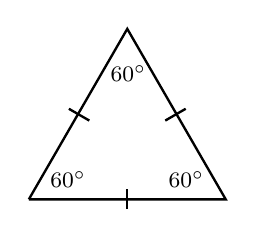
\begin{tikzpicture}[scale=2.5]
	\draw[line width= 0.03cm] (0,0) -- (1,0) -- (0.5,0.866) -- (0,0);
	\draw[line width= 0.03cm] (0.5,-0.05) -- (0.5,0.05);
	\draw[line width= 0.03cm] (0.69282, 0.4) -- (0.796743, 0.46);
	\draw[line width= 0.03cm] (0.30718, 0.4) -- (0.203257, 0.46);
	\node at (0.2,0.1) {\footnotesize$60^\circ$};
	\node at (0.8,0.1) {\footnotesize$60^\circ$};
	\node at (0.505,0.64) {\footnotesize$60^\circ$};
	\end{tikzpicture}
	\] \pvspace{1.3cm}



% Quiz 14
\quizsol \textit{True/False}: Two geometric figures are congruent if and only if they have the same area. \pspace

\sol The statement is \textit{false}. Certainly, if two geometric figures are congruent, they must have the same area. However, just because two geometric figures have the same area does not mean that they are congruent. For example, certainly no triangle and square can be congruent---they have different number of sides. However, consider a triangle and square with the same base length but the triangle has twice the height, as shown below.
	\[
	\fbox{
	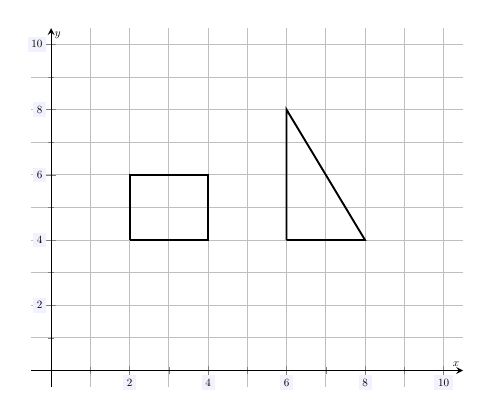
\begin{tikzpicture}[scale=0.8,every node/.style={scale=0.5}]
	\begin{axis}[
	grid=both,
	axis lines=middle,
	ticklabel style={fill=blue!5!white},
	xmin= -0.5, xmax=10.5,
	ymin= -0.5, ymax=10.5,
	xtick={0,2,...,10},
	ytick={0,2,...,10},
	minor x tick num = 1,
	minor y tick num = 1,
	xlabel=\(x\),ylabel=\(y\),
	]
	\draw[line width=0.03cm] (2,4) -- (4,4) -- (4,6) -- (2,6) -- (2,4);
	\draw[line width=0.03cm] (6,4) -- (8,4) -- (6,8) -- (6,4);
	\end{axis}
	\end{tikzpicture}
	}
	\] 
Then the area of the square are\dots
	\[
	\begin{aligned}
	A_\square&= s^2= 2^2= 4 \\[0.3cm]
	A_\Delta&= \frac{1}{2}\,bh= \frac{1}{2} \cdot 2 \cdot 4= 4
	\end{aligned}
	\]
Therefore, there are geometric figures with have the same area but are not congruent. 



\newpage



% Quiz 15
\quizsol \textit{True/False}: Suppose you have a triangle, $\Delta ABC$, such that the sides $\overline{AB}$, $\overline{BC}$, and $\overline{AC}$ are such that $|\overline{AB}| < |\overline{BC}| < |\overline{AC}|$. Then we have $|\overline{AB}|^2 + |\overline{BC}|^2= |\overline{AC}|^2$. \pspace

\sol The statement is \textit{false}. The series of inequalities $|\overline{AB}| < |\overline{BC}| < |\overline{AC}|$ simply states that $\overline{AB}$ has the shortest length, $\overline{BC}$ is the `medium' length side, and $\overline{AC}$ is the side with the greatest length, i.e. the hypotenuse. But then $\overline{AB}$ and $\overline{BC}$ are the legs of this right triangle with hypotenuse $\overline{AC}$. Then the equation $|\overline{AB}|^2 + |\overline{BC}|^2= |\overline{AC}|^2$ is the Pythagorean Theorem. However, the Pythagorean Theorem holds if and only if $\Delta ABC$ is a right triangle, which we are not told. Certainly, there exist non-right triangles. Therefore, this relation is not generally true. 




































\end{document}